\documentclass[12pt]{article}
\usepackage{pgf, tikz}
\usepackage{amsmath, amsfonts, amssymb, graphicx}
\usepackage{subfig}
\usepackage{float}
\usepackage[utf8]{inputenc}
\usepackage[spanish]{babel}
\usepackage{amsthm}

\setlength{\textheight}{23cm} \setlength{\evensidemargin}{0cm}
\setlength{\oddsidemargin}{-.5cm} \setlength{\topmargin}{-3cm}
\setlength{\textwidth}{17.5cm} \setlength{\parskip}{.2cm}


%opening

\begin{document}
	\begin{picture}(80, 80)
	\put(170,0){\hbox{
\includegraphics[scale=0.6]{cimat_logo.png}}}
	\end{picture}
	
	\begin{center}
		\begin{huge}
			Centro de Investigación en Matemáticas, A.C.
		\end{huge}
	\end{center}

	\begin{center}
		\begin{large}
			Descripción tarea - Métodos numéricos
		\end{large}
	\end{center}
	
	\begin{center}
		\textbf{Erick Salvador Alvarez Valencia}
	\end{center}

	\begin{center}
		15 de Octubre de 2017
	\end{center}



%\maketitle

%\tableofcontents

\section{Aproximación de una función por mínimos cuadrados}

\subsection{Descripción}
El método a describir es la aproximación de una función, en este caso de grado dos (una parábola) por medio del método de mínimos cuadrados, el cual, dado un conjunto de puntos ${(x_i, y_i)_{i=1}^{m}}$ podemos encontrar la función que mejor se aproxime a ellos por medio de una minimización del error $||Ax=y||$ donde $A$ es una matriz que contiene familias de funciones, $x$ contiene los coeficientes desconocidos y $y$ las ordenadas de los puntos anteriormente definidos.\\
La idea de este método es que una vez tengamos definido el sistema a minimizar sus error, obtengamos su gradiente y lo igualemos a cero, para lo cual llegaremos a la siguiente igualdad: $E(a, b, c) = \sum_{i=1}^{m}E_{i}^{2} = ||Ax-y||$ y finalmente llegando a: $\nabla E = 0 \Rightarrow A^T Ax = A^T y$. Al resolver ese sistema podremos encontrar el vector $x$ el cual contiene los coeficientes de la mejor aproximación a la función de grado dos. Queda notar que esto se puede extender a polinomios de grado $n$.

\subsection{Ejemplo de ejecución}
A continuación se mostrará el resultado de la ejecución del método de mínimos cuadrados donde los puntos $(xi, yi)$ fueron generados usando medio ciclo de la función seno, y con una discretización de 50 puntos.\\

\begin{figure}[H]
	\centering
	\subfloat[][Figura 1. Resultados de la aproximación por mínimos cuadrados.]{
		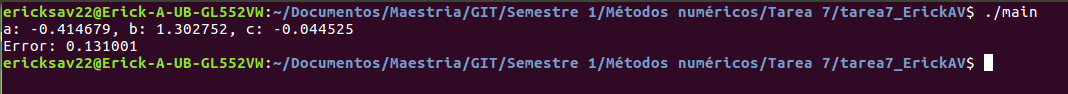
\includegraphics[scale=0.4]{E1.png}
	}\hfill
\end{figure}

En la Figura 1. podemos observar que el programa nos arroja los coeficientes de la parábola que mejor se ajusta a los puntos generados. De la misma forma también se muestra el error entre los $y_i$ y los $f(x_i)$ donde $f(x)$ es la función encontrada.\\

Para una mejor ejemplificación se mostrará una gráfica de los resultados anteriores.\\

\begin{figure}[H]
	\centering
	\subfloat[][Figura 2. Función generada (seno) en contra de la función encontrada (parábola).]{
		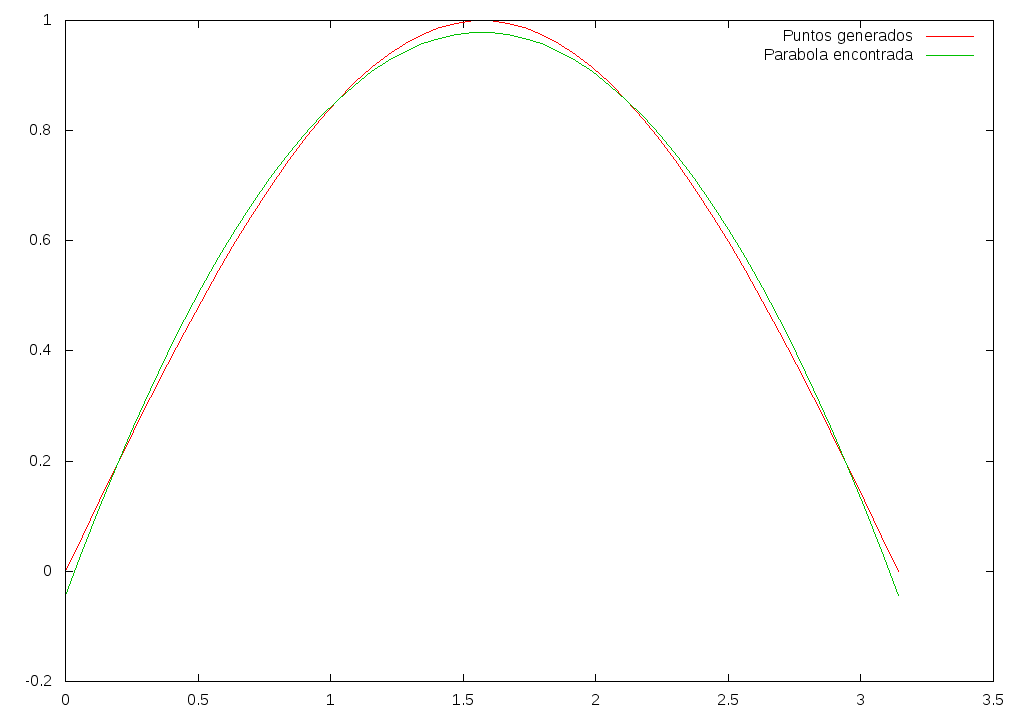
\includegraphics[scale=0.4]{Grafica.png}
	}\hfill
\end{figure}

\subsection{Compilación y ejecución}
\textbf{Para compilar:} En la carpeta encontraremos los archivos $.c$ y $.h$ con los que se podrá compilar el ejecutable. De la misma forma, en conjunto con los archivos anteriores, también podremos encontrar un Makefile para, en caso de encontrarse en linux, compilar de manera sencilla.

\begin{enumerate}
	\item \textbf{Compilar usando Makefile:} En la terminal, nos colocamos en el directorio donde se encuentre el programa, y ejecutamos el comando $make$, automáticamente se realizará la compilación y se generará el ejecutable. El Makefile también contiene el comando $make\ clean$ el cual limpiará los archivos generados por la compilación, incluyendo el ejecutable.
	\item \textbf{Compilar directamente:} De la misma forma, podemos compilar directamente usando los siguientes comandos (en terminal):
	\begin{itemize}
		\item gcc -c main.c
		\item gcc -c memo.c
		\item gcc -c matriz\_vector.c
		\item gcc -c met\_num.c
		\item gcc -o main main.o memo.o matriz\_vector.o met\_num.o -lm
	\end{itemize}
\end{enumerate}

\textbf{Para ejecutar:} Únicamente debemos de usar el comando $./main$ para ejecutar el programa en consola, este no recibe argumentos.\\
El programa imprimirá los coeficientes $a$, $b$, y $c$ encontrados, el error generado por las funciones, y un archivo de texto con los puntos $x_i$, $y_i$ y $f(x_i)$ mediante el cual se generó el gráfico con GNUplot.
\end{document}
